\section{Results and discussion}
\label{sec:resultsAndDiscussion}
In this section, 
we present how well the proposed RNO based potential formulated friction can fit the original rate-and-state friction, 
and also whether or not it facilitates implicit solution of dynamic problems through solving the spring slider example. 
\subsection{Fitting results to original rate-and-state friction}
After 100 epochs of training under the optimal Neural Network structure given by OPTUNA, 
the RNO potentials are able to fit the original rate-and-state sequences well. 
Figure~\ref{fig:19thAnd99thRSNN} shows the fitting results of the two example sequences early mentioned in Figure~\ref{fig:19thAnd99thRS}. 
Note that these two sequences are in the test dataset and have not been used for training the potentials. 
After training of the potentials $W_{NN}, D^\dagger_{NN}$ and $D^*_{NN}$, 
we can obtain $f^{NN}$s that are fairly close to $f^{RS}$s. 
Table~\ref{tab:dimXi} confirms that the error between $f^{NN}$ and $f^{RS}$ is small, 
and that there needs to be at least $1$ hidden variable ($\dim(\bm{\xi})$) to achieve small error. 
Since further increasing the number of hidden variables does not reduce the error, 
the results shown next are all based on $\dim(\bm{\xi}) = 1$. 
The fact that it suffices to use $\dim(\bm{\xi}) = 1$ makes intuitive sense since the original rate-and-state friction has only one state variable $\theta$. 

Due to limited access to experimental data with the same rate-and-state friction properties, 
we cannot compare the error of $f^{RS}$ and $f^{NN}$ both fitted to 
experimental sequences $f^{EXP}$. 
We here include a typical rate-and-state fitted experimental sequence from (Kim et al., in preparation, 2024), 
which is shown by Figure~\ref{fig:RSVsExp}. 
The best fit rate-and-state sequence achieves an relative $L_2$ error of $0.0268$, 
which is two orders of magnitude higher than the average relative $L_2$ of fitting $f^{NN}$ to $f^{RS}$. 
This implies that the fitting error between $f^{NN}$ and $f^{RS}$ is negligible compared with fitting $f^{RS}$ to noisier $f^{EXP}$, 
and thus $f^{NN}$ has comparable ability to explain the history dependencies in the empirical observations. 

\begin{figure}[htbp]
    \centering
    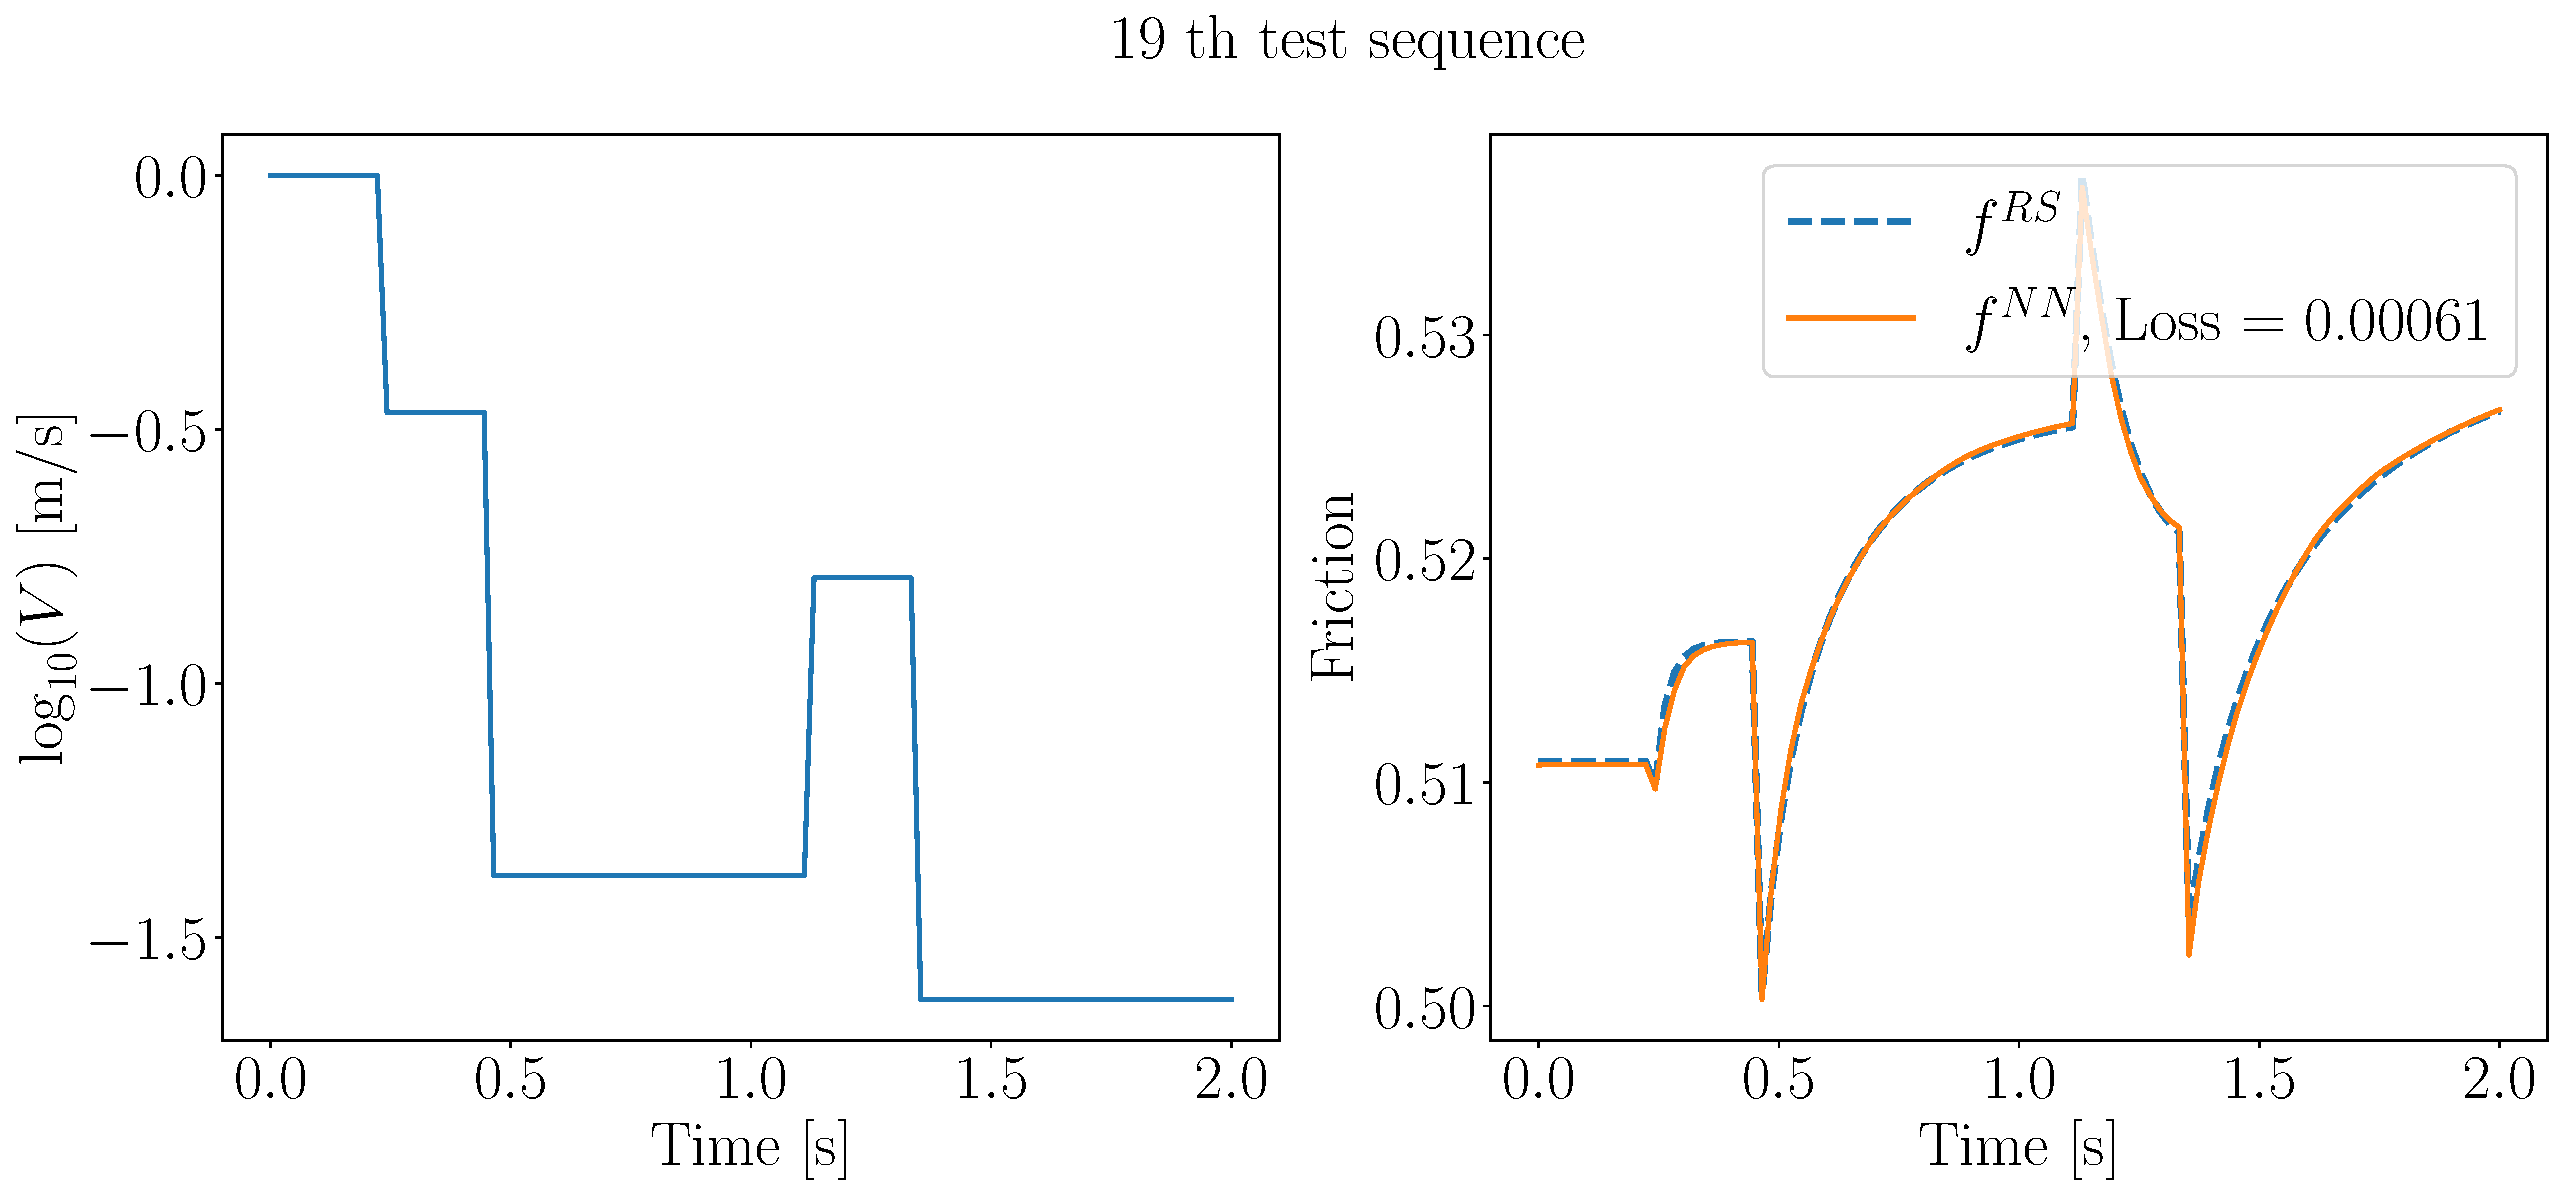
\includegraphics[height=0.3\textheight]{figures/19thRSNN.pdf}
    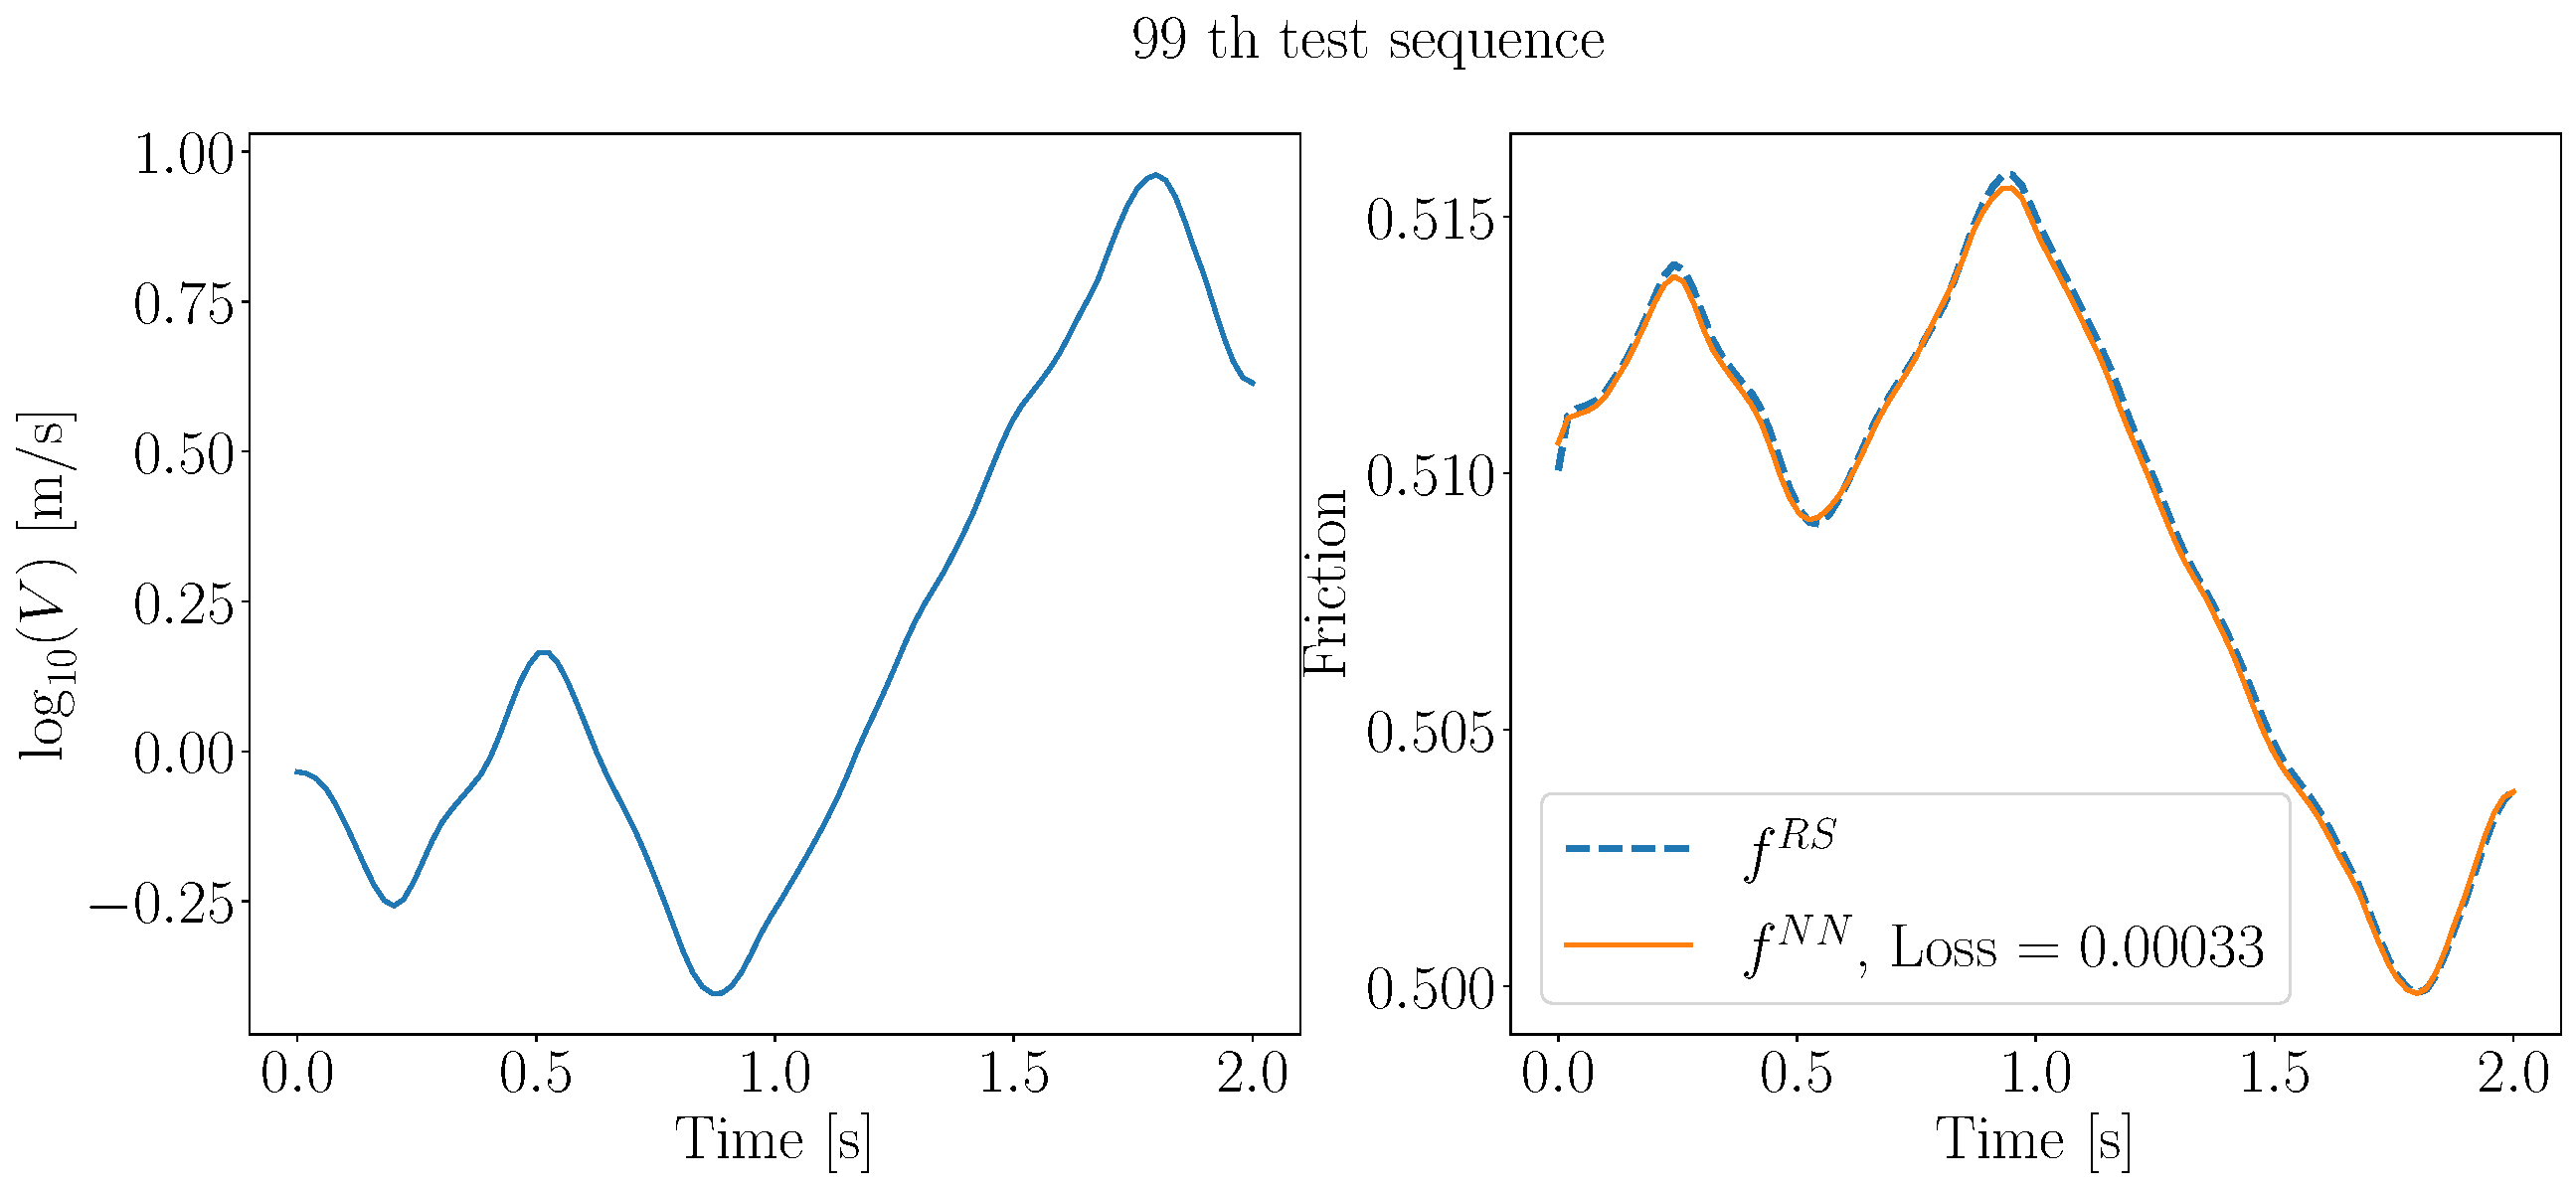
\includegraphics[height=0.3\textheight]{figures/99thRSNN.pdf}
    \caption{Examples of trained $f^{NN}$ vs. $f^{RS}$ for both velocity jump (upper) and continuous variation (lower) sequences. 
    Loss here refers to relative $L_2$ error as defined by (\ref{eq:relativeLpError}). 
    These two sequences are from the test dataset and are not used for training the potentials.}
    \label{fig:19thAnd99thRSNN}
\end{figure}

\begin{figure}[htbp]
    \centering
    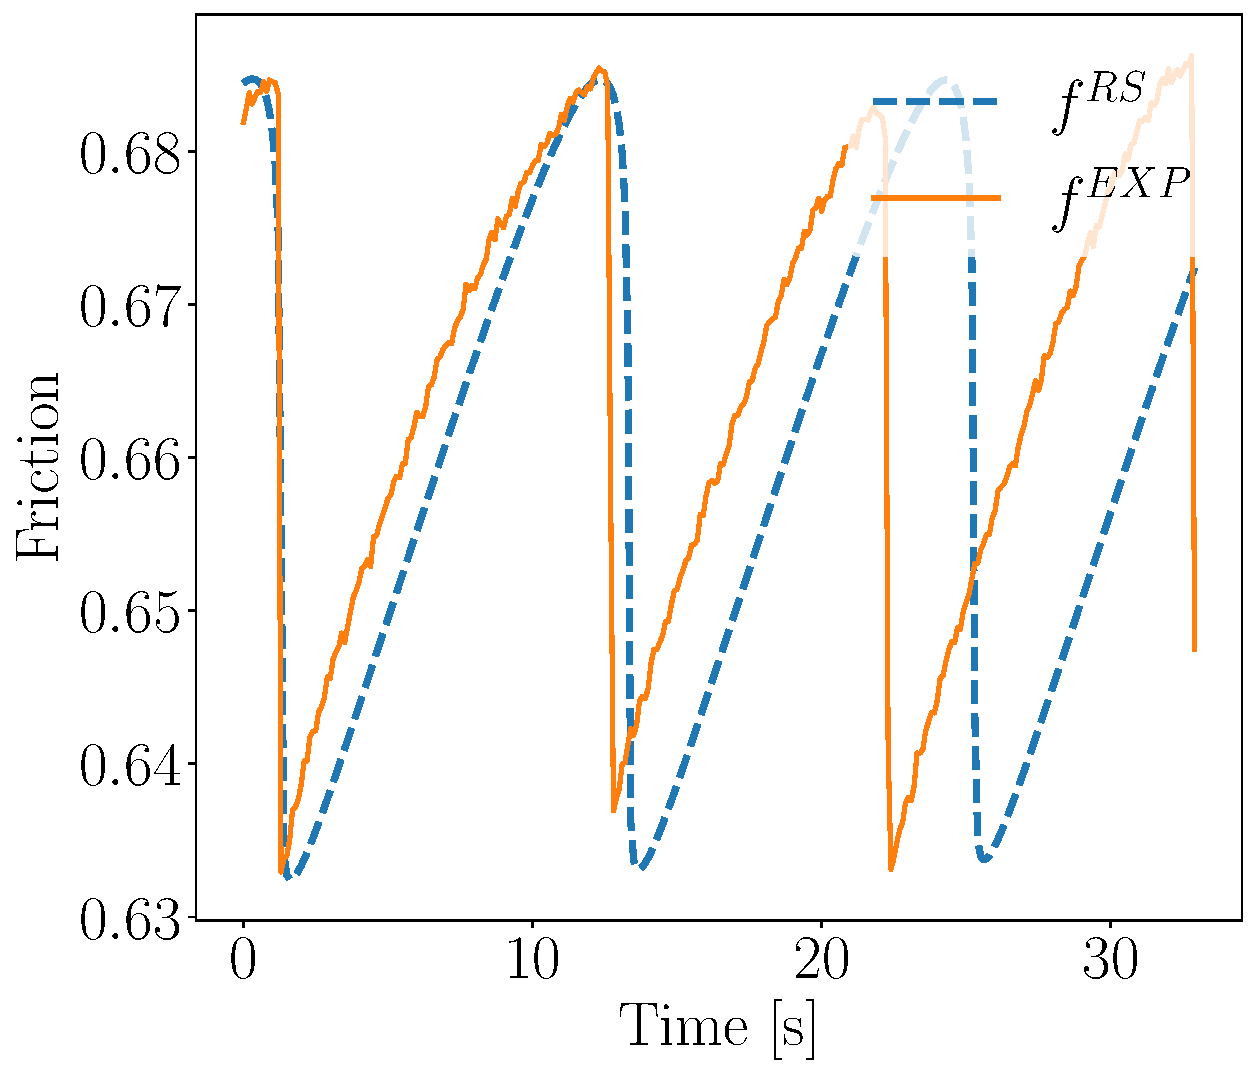
\includegraphics[width=0.4\textwidth]{figures/RSVsExp.pdf}
    \caption{A typical fit of rate-and-state friction to experimental data, 
    the relative $L_2$ error of $f^{RS}$ against $f^{EXP}$ is 0.0268. 
    Data provided by Taeho Kim.}
    \label{fig:RSVsExp}
\end{figure}

\begin{table}[htbp]
    \centering
    \begin{tabular}{cccc}
        \hline
        $\dim(\bm{\xi})$ & 0 & 1 & 2 \\
        \hline
        Training error ($L_2$) & 0.18 $\pm$ 0.01 & 0.0004 $\pm$ 0.0004 & 0.0007 $\pm$ 0.0006\\
        Testing error ($L_2$) & 0.18 $\pm$ 0.01 & 0.0005 $\pm$ 0.0004 & 0.0007 $\pm$ 0.0006 \\
        \hline
    \end{tabular}
    \caption{Training and testing relative $L_2$ error for $\dim(\bm{\xi}) = 0, 1, 2$, 
    averaged over 160 test sequences. 
    Error decreases significantly after introducing one hidden variable $\dim(\bm{\xi}) = 1$, 
    while introducing more hidden variables do not further reduce the error. }
    \label{tab:dimXi}
\end{table}

\subsection{The trained potentials $W, D^\dagger$ and $D^*$}
To make (\ref{eq:JfunctionalMin}) a convex minimization problem, 
we need to confirm convexity of $J$ in $(x, \xi)$. 
Figure~\ref{fig:WAndD} shows that the learnt $W$ is linear in $x$, 
and thus also convex. 
The fact that $W$ is linear makes sense because of material frame indifference.   
$D^*$ is convex in $\dot{d}$, 
which is consistent with its definition as the Legendre transform of $D$. 
Figure~\ref{fig:Ddagger} plots $D^\dagger(\dot{x}, \xi)$, 
and it is not convex because $\partial^2 D^\dagger / \partial \dot{x}^2 < 0$. 
To ensure convexity of $J$ in $(x, \xi)$, 
we need the Hessian of $J$ to be positive semi-definite for all $(x, \xi)$, 
which ends up posing a constraint on $\Delta t$: 
\begin{align}
    &1 \cdot m + \Delta t \left(\frac{\partial^2 D^\dagger}{\partial \dot{x}^2}\right) + O(\Delta t^2)  &\ge 0, \label{eq:PSD1}\\
    & 1 \cdot m \frac{d^2D}{d\dot{\xi}^2} 
    + \Delta t \left(\frac{\partial^2 D^\dagger}{\partial \dot{x}^2} \frac{d^2D}{d\dot{\xi}^2} + m \frac{\partial^2 D^\dagger}{\partial \xi^2}\right) 
    &\notag \\
    & + \Delta t^2 \left[\left(k + \frac{d^2W}{dx^2}\right)\frac{d^2D}{d\dot{\xi}^2} + \frac{\partial^2 D^\dagger}{\partial \dot{x}^2}\frac{\partial^2 D^\dagger}{\partial \xi^2}-\frac{\partial^2D^\dagger}{\partial \dot{x} \partial \xi}\right] 
    &\notag \\
    & + \Delta t^3 \left[\left(k + \frac{d^2W}{dx^2}\right)\frac{\partial^2D^\dagger}{\partial \xi^2}\right] & \ge 0. \label{eq:PSD2}
\end{align}

Equation (\ref{eq:PSD1}) can be satisfied with $\Delta t$ smaller than an upper bound, 
since then the $m$ term will dominate even if $\partial^2 D^\dagger / \partial \dot{x}^2 < 0$. 
(\ref{eq:PSD2}) also reduces to an upper bound constraint on $\Delta t$, 
since $d^2 D / d \dot{\xi}^2 > 0$ based on the assumption. 
In practical it is also convex because it is the Legendre transform of the learnt $D^*(\dot{d})$. 


\begin{figure}[htbp]
    \centering
    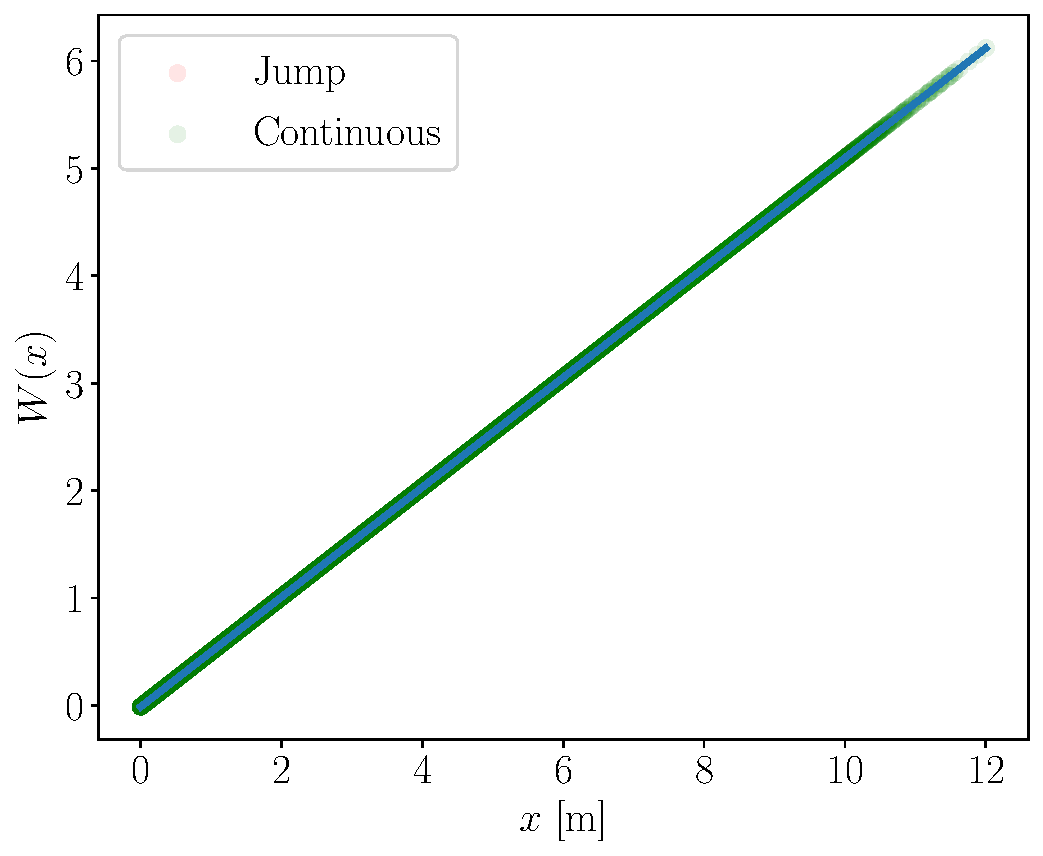
\includegraphics[height=0.25\textheight]{figures/Trial0216_combined_800_W.pdf}
    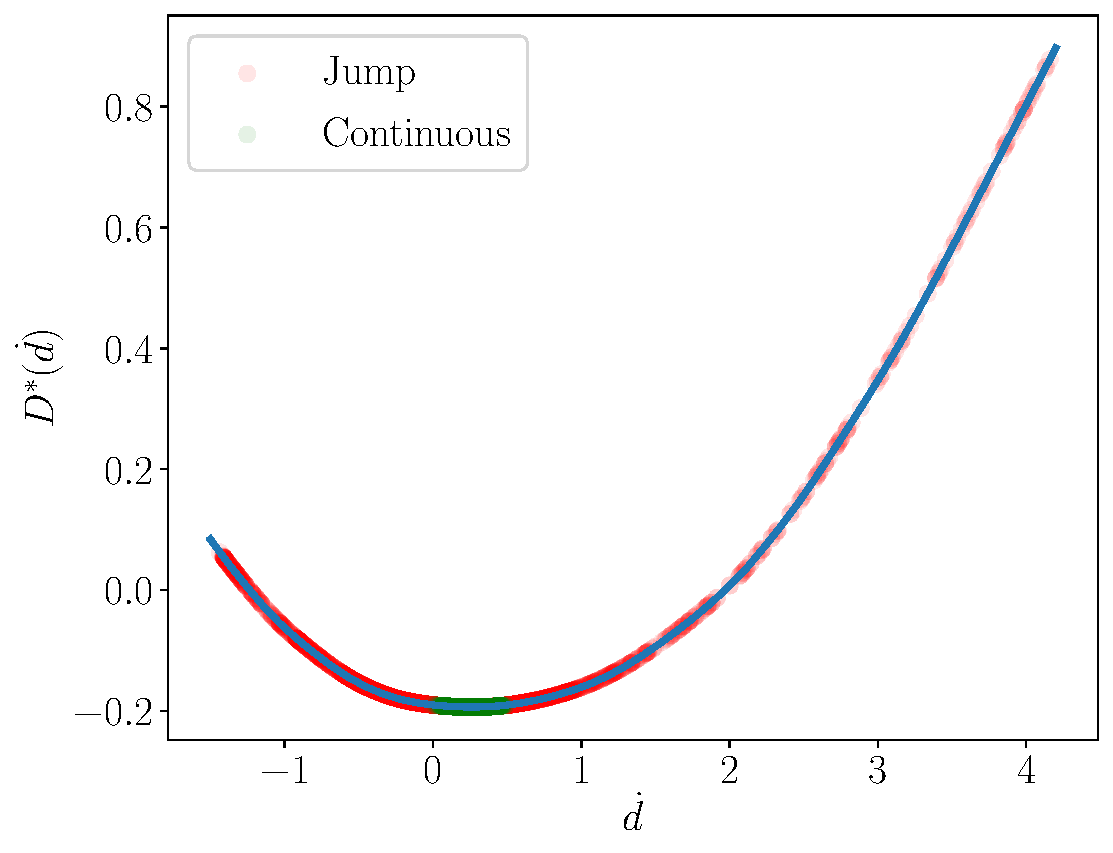
\includegraphics[height=0.25\textheight]{figures/Trial0216_combined_800_D_star.pdf}
    \caption{Learnt $W(x)$ (left) and $D^*(\dot{d})$ (right). 
    $W$ is linear in $x$ corresponding to the reference friction coefficient, 
    $D^*$ is convex, 
    which complies with the definition as the Legendre transform of $D$.}
    \label{fig:WAndD}
\end{figure}
\begin{figure}[htbp]
    \centering
    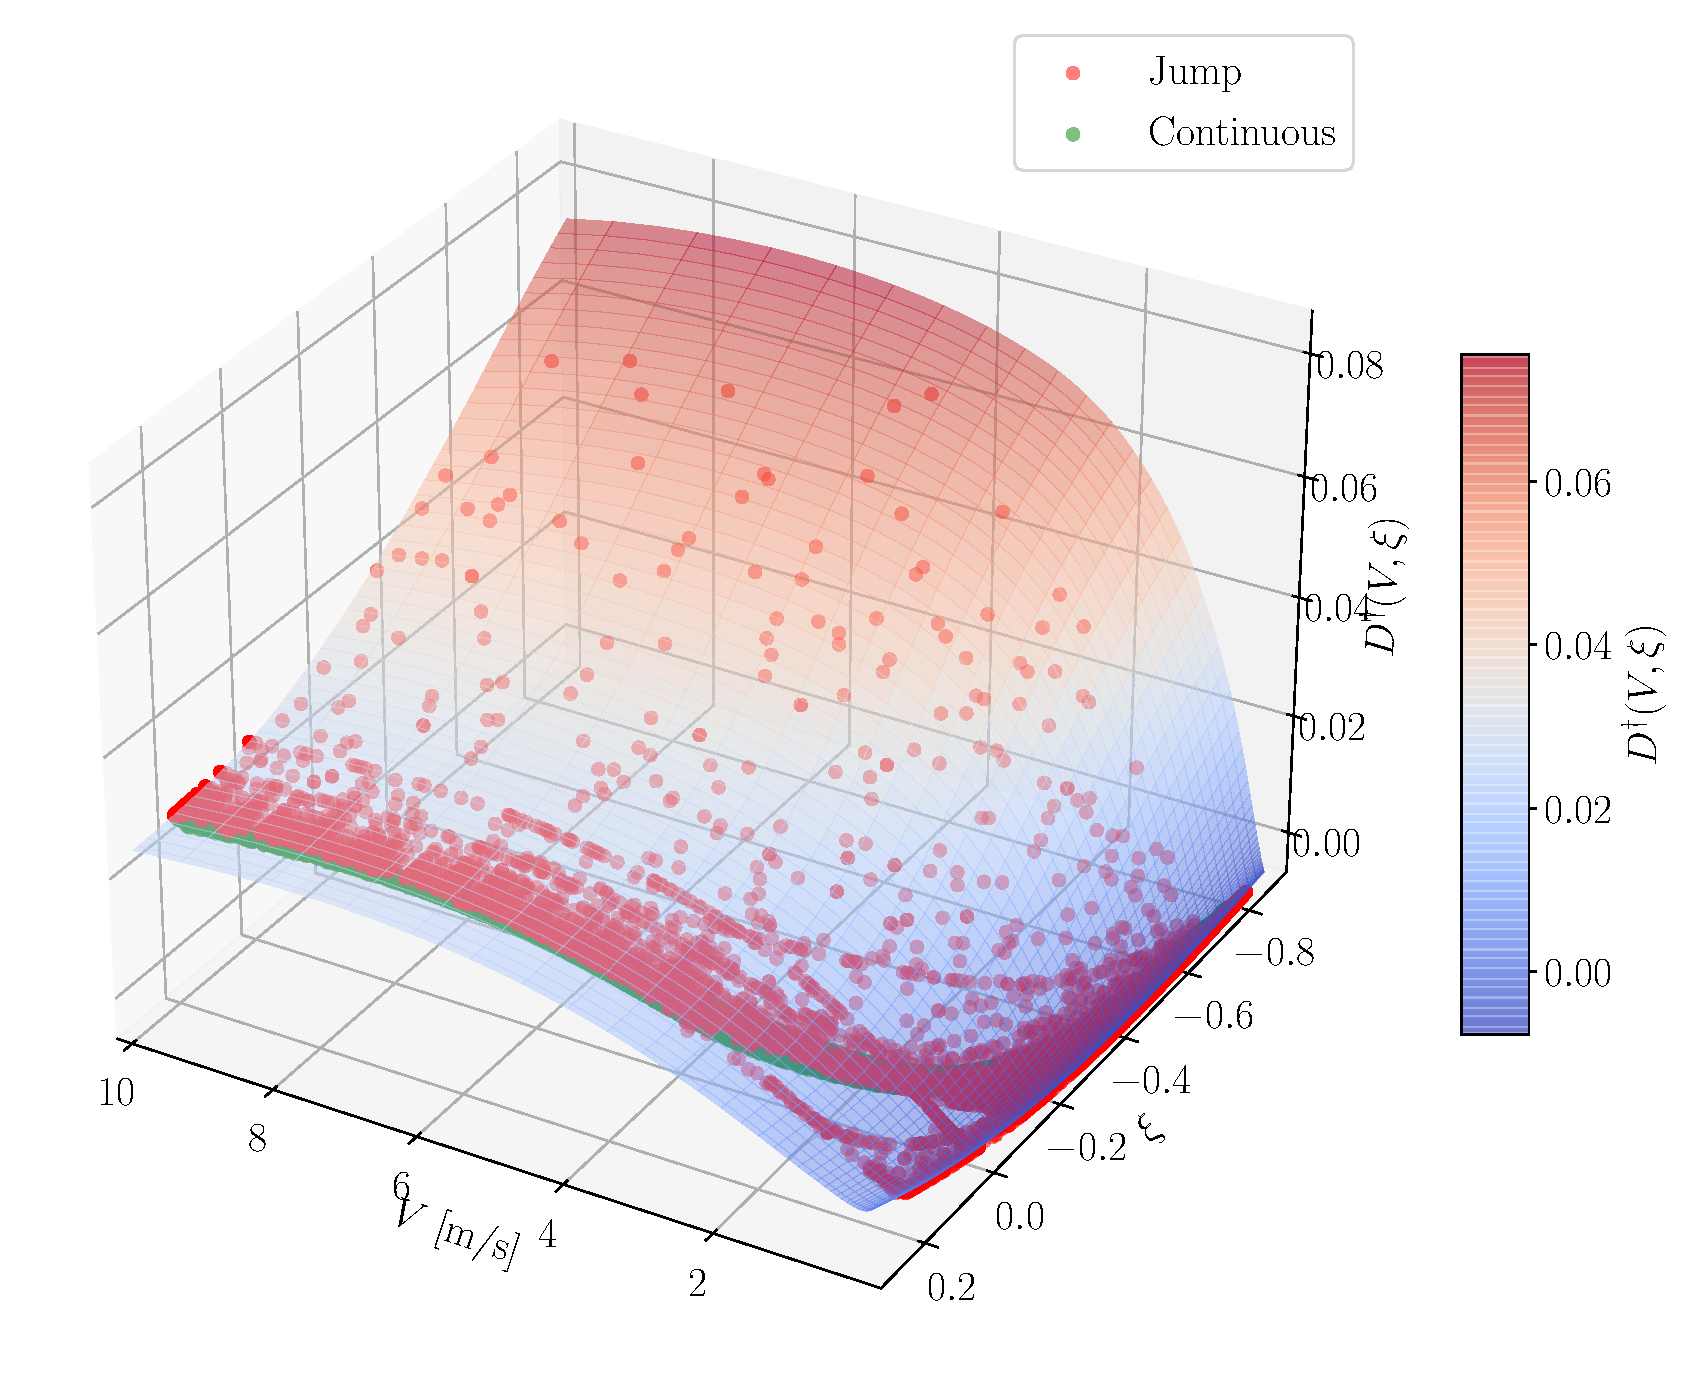
\includegraphics[height=0.5\textheight]{figures/Trial0216_combined_800_D_dagger_normal.pdf}
    \caption{Learnt $D^\dagger(\dot{x}, \bm{\xi})$, 
    $D^\dagger$ is not convex in $(\dot{x}, \xi)$.
    The red dots show the trajectories of velocity-jump dataset, 
    while the green dots show the trajectories of continuous variation dataset.}
    \label{fig:Ddagger}
\end{figure}

In summary, 
we find that of the three learnt potentials, 
$W$ is linear in $x$, 
consistent with material-frame indifference; 
$D^*$ is convex in $\dot{d}$, 
consistent with its definition by Legendre transform; 
while $D^\dagger$ is not convex in $(\dot{x}, \xi)$. 
However, 
one can still achieve convexity of $J(x, \xi)$ in (\ref{eq:Jfunctional}) with an upper bound constraint on $\Delta t$, 
and thus it is legitimate to write (\ref{eq:JfunctionalMin}) as a convex minimization problem. 

\subsection{Uniqueness of the hidden variable $\xi$}
One important property of the hidden variable $\xi$ is that since we cannot attach a concrete physical meaning to it, 
it is possibly non-unique. 
In practice, 
even different training runs can possibly lead to different $\xi$'s that all fit the training dataset well. 
However, 
in our potential formulation an underlying assumption is that $D$ is only a function of $\dot{\xi}$. 
Then if there exists $\eta = f(\xi)$ as a different hidden variable with $f$ and $f^{-1}$ being smooth, 
we have 
\begin{align}
    D^\eta\left(\dot{\eta}\right) = D^\eta\left(f'(\xi)\dot{\xi}\right) = D^\xi \left(\dot{\xi}\right) \label{eq:uniqueXi}, 
\end{align}
which implies that $f'(\xi)$ is a constant, 
and thus $\xi$ is unique up to affine transformations. 

We verify the above-discussed uniqueness of $\xi$ by training three different models on three datasets generated similarly using the same rate-and-state friction model. 
Then we obtain the trajectories of $\xi$s of the three trained model on the same test dataset. 
After performing linear regression of $\xi^{(3)}$ and $\xi^{(2)}$s on $\xi^{(1)}$, 
i.e. the hidden variable from the first trained model, 
we check their regression coefficient as a reflection of how linearly correlated the $\xi$s are. 

\begin{figure}[htbp]
    \centering
    \includegraphics[width=0.9\textwidth]{figures/nonuniqueXis.pdf}
    \caption{Linear regression of $\xi^{(3)}$ and $\xi^{(2)}$s on $\xi^{(1)}$. 
    Red and green dots are the data points while the solid lines are the regression result.
    $(0, 0)$ should be a fixed point since all sequences start with $\xi = 0$ as their initial condition.}
    \label{fig:nonuniqueXis}
\end{figure}

Figure~\ref{fig:nonuniqueXis} shows that the regression coefficient is $>0.98$ and thus the different $\xi$s are indeed unique up to linear transform.


\subsection{Example: solving spring slider under displacement control loading}
As stated above, 
the potential formulated friction should facilitate implicit solution of dynamic initial value problems, 
because advancing the solution to the next time step can be written as a convex minimization problem given by (\ref{eq:JfunctionalMin}). 
Here we try to verify that by considering the spring-slider problem with displacement-control loading. 
As shown by Figure~\ref{fig:springslider}, 
friction between the mass block and the ground is modeled with either original rate-and-state friction or trained potentials with the same rate-and-state properties. 
We testify the two friction formulations with both explicit (4th order Runge Kutta) and implicit (Adams) solvers trying to solve the same spring-slider problem. 
The solvers are imported from a standard ODE solver package torchdiffeq \cite{torchdiffeq}.
Spring constant $k$ is randomly sampled within a range that covers both $k < k_{crit}$ and $k > k_{crit}$, 
where $k_{crit}$ is the critical stiffness for unstable stick-slip events to happen under constant loading speed $\dot{x}_p(t)$ \cite{rice_stability_1983, Gu_Rice_1984}. 
and we create a dataset of 77 loading sequences with different velocity-jump-like $x_p(t)$s. 

We first notice that since the training dataset of the potentials does not include these spring-slider sequences of $V(t), f(t)$, 
the error between the potential friction and
the original rate-and-state friction is large. 
To resolve this, 
we generate $200$ sequences from solving the spring-slider problem with rate-and-state friction and different loadings, 
and further train our potentials on these $200$ sequences for $400$ epochs. 
Indeed the further-trained NN potentials (denoted as NN') reduce the error between $f^{NN'}$ and $f^{RS}$ when solving spring-slider sequences. 

Table~\ref{tab:NNvsNNPrime} shows that after further training the potentials on spring-slider solutions by rate-and-state friction, 
the relative $L_2$ error on $x(t), \dot{x}(t), f(t)$ decreases by more than $50\%$. 
Figure~\ref{fig:SSseq8} plots an example spring-slider sequence. 
It is clear that further trained NN' agrees better with the solution obtained by the original rate-and-state friction. 
Another example sequence is shown by Figure~\ref{fig:SSseq9}.
The results and discussions next will all be based on the solution of NN'. 

\begin{figure}[htbp]
    \centering
    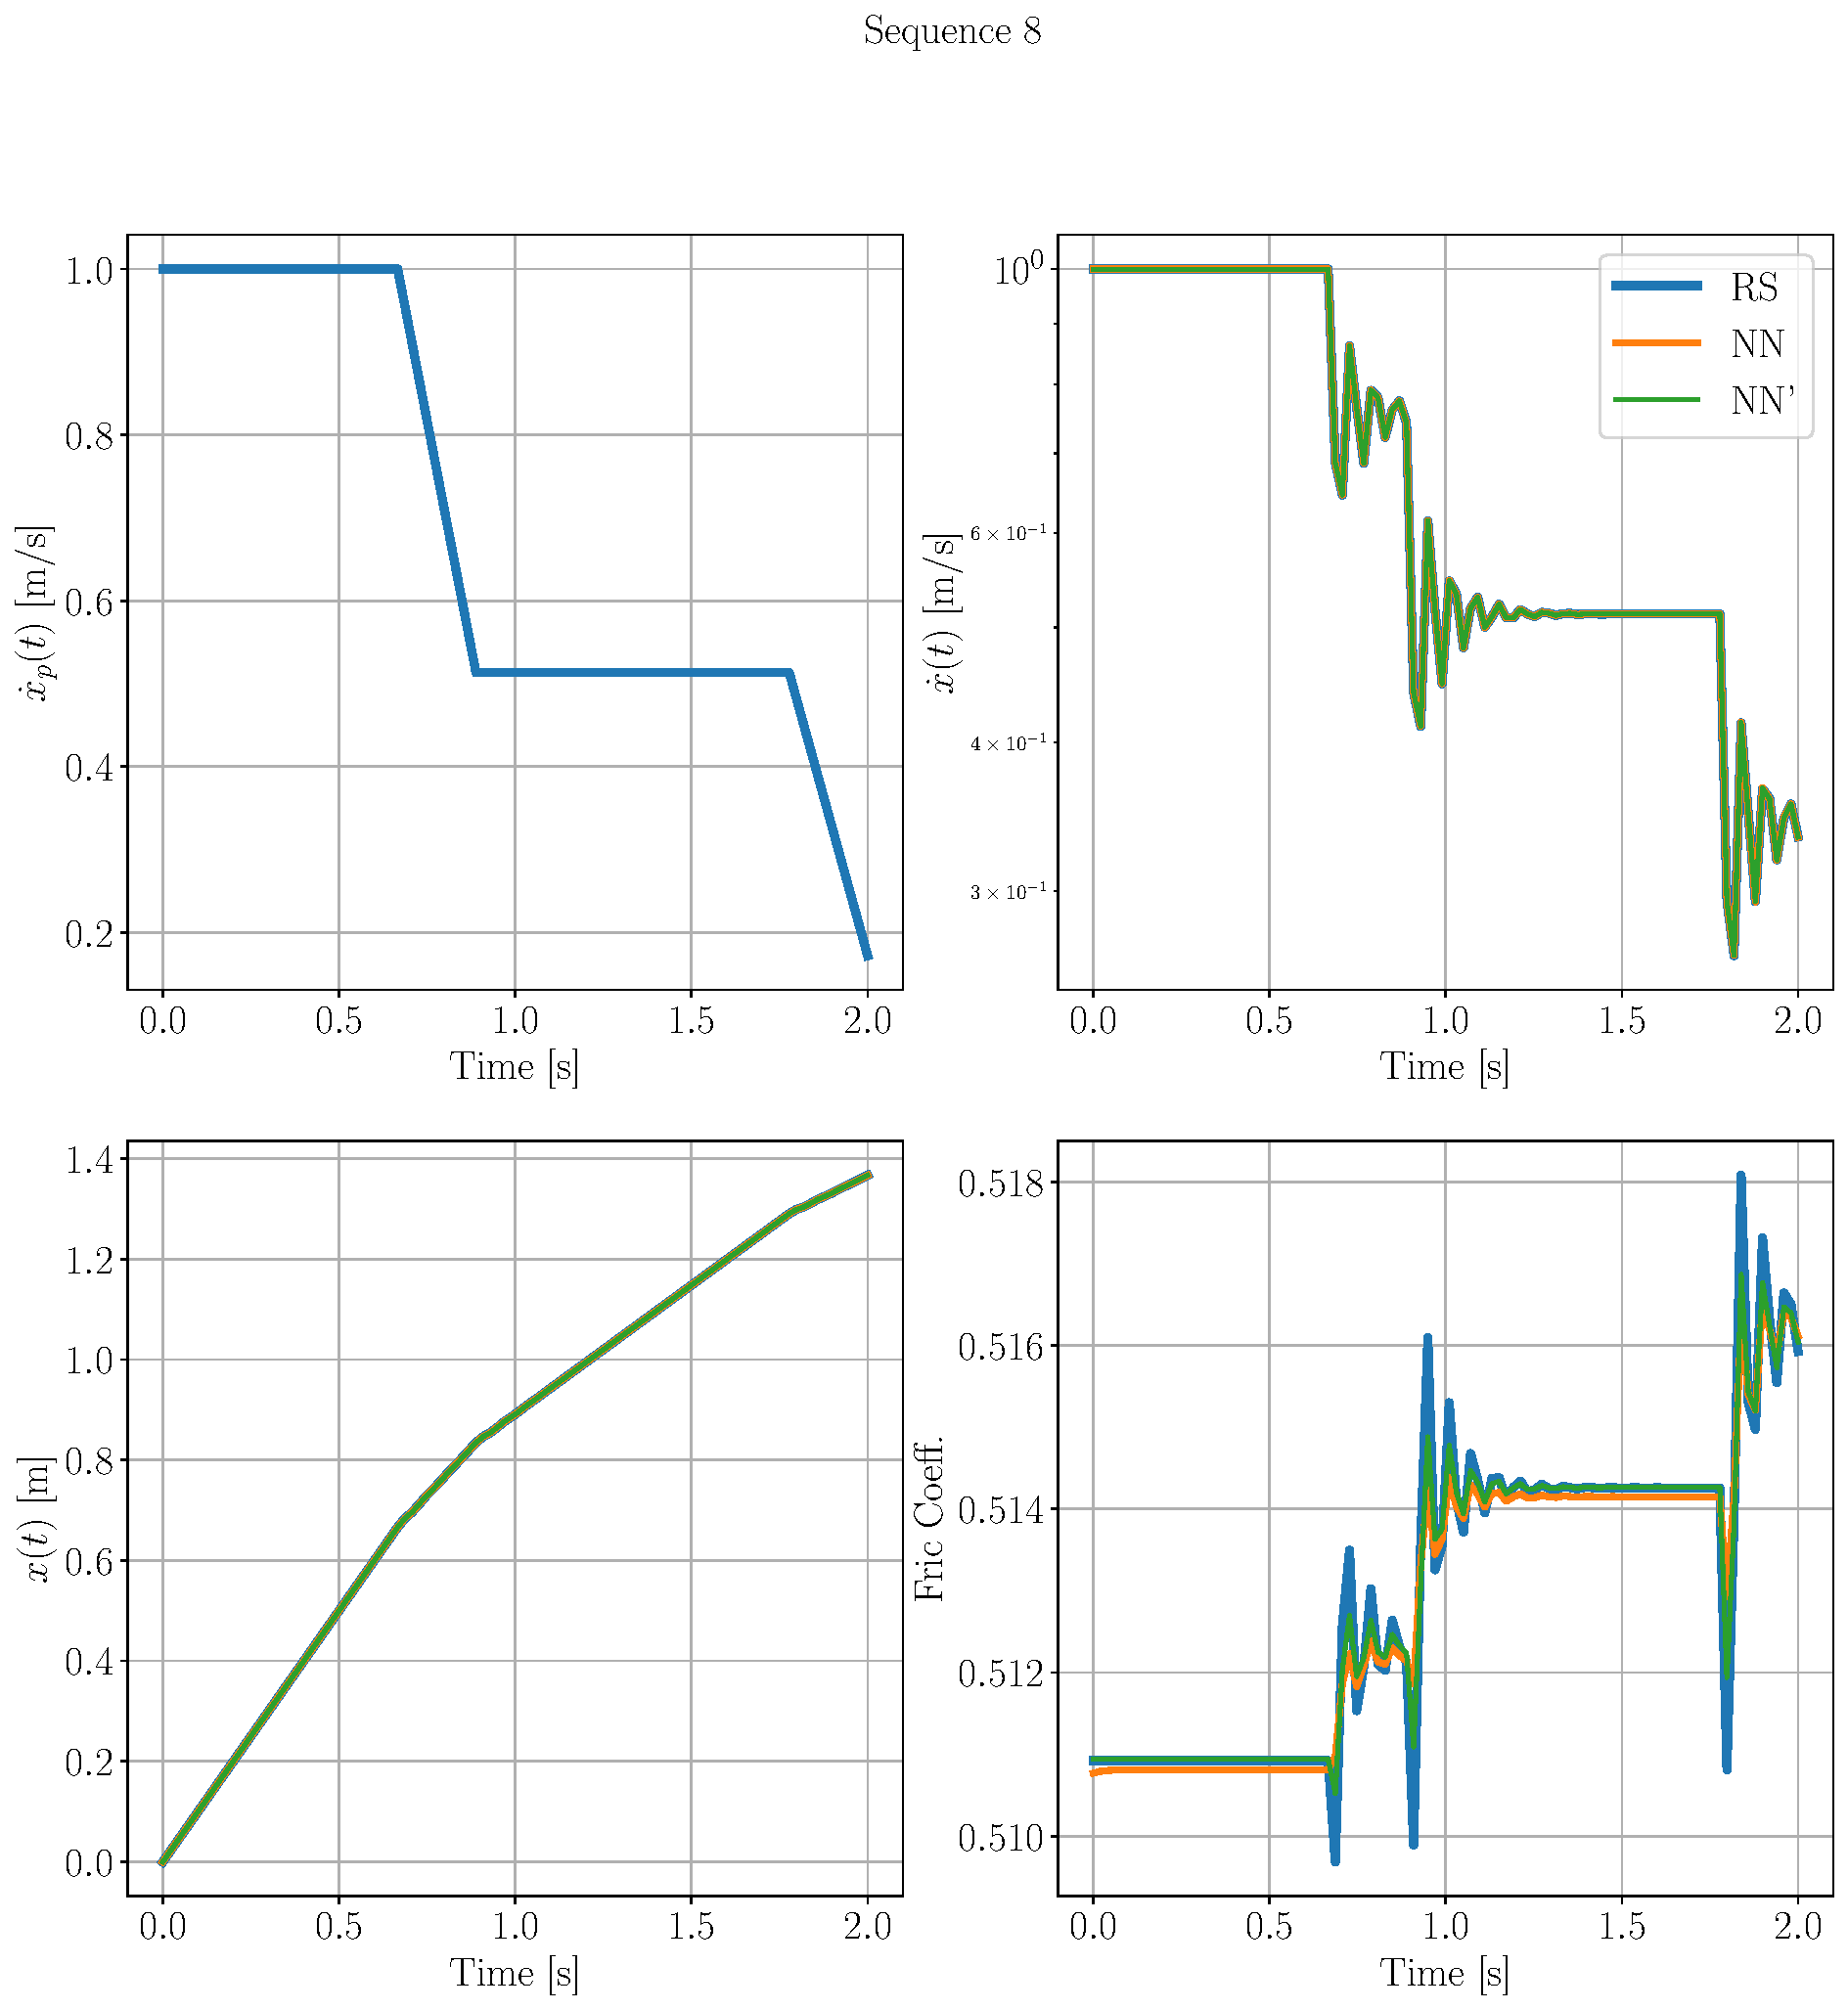
\includegraphics[width=0.9\textwidth]{figures/SS_seq8_0216_0521SS_combined_800.pdf}
    \caption{An example sequence of spring-slider solution with original rate-and-state friction, 
    NN potentials, 
    and NN potentials further trained on spring-slider sequences}
    \label{fig:SSseq8}
\end{figure}

\begin{table}[htbp]
    \centering
    \begin{tabular}{ccc}
        \hline
        Solution term & NN & NN' \\
        \hline
        $x(t)$ & $(1.9 \pm 1.8)\times 10^{-5}$ & $(5.4 \pm 4.4 )\times 10^{-6}$\\
        $\dot{x}(t)$ & $(2.7 \pm 3.6)\times 10^{-4}$ & $(1.6 \pm 2.2)\times 10^{-4}$\\
        $f(t)$ & $0.030 \pm 0.024$ & $0.016 \pm 0.016$\\
        \hline
    \end{tabular}
    \caption{Testing relative $L_2$ error for the original potentials only trained on velocity-jump and continuous variation dataset (NN), 
    updated potentials further trained on 200 spring-slider like dataset (NN'). 
    averaged over 10 test spring-slider sequences. }
    \label{tab:NNvsNNPrime}
\end{table}

The potential formulated friction is that it can solve all the sequences, 
with either explicit or implicit solver.  
In contrast the original rate-and-state friction fails to solve over $60\%$ of the sequences at even the finest $\Delta t$ with the implicit solver, 
and over $40\%$ with the explicit solver. 
Table~\ref{tab:NaNRatioSpringSliderRsVsNNRespective} lists the ratio of sequences that cannot be solved by each (NN/RS, ex/implicit) pair. 

\begin{table}[H]
    \centering
    \begin{tabular}{cccccccc}
        \hline
        $\Delta t$ [s] & $2^{-13.5}$ & $2^{-13.0}$ & $2^{-12.5}$ & $2^{-12.0}$ & $2^{-11.5}$ & $2^{-11.0}$ \\
        \hline
        NN, implicit & 0.000 & 0.000 & 0.000 & 0.000 & 0.000 & 0.000 \\
        NN, explicit & 0.000 & 0.000 & 0.000 & 0.000 & 0.000 & 0.000 \\
        RS, implicit & 0.506 & 0.571 & 0.623 & 0.623 & 0.675 & 0.727 \\
        RS, explicit & 0.455 & 0.455 & 0.455 & 0.455 & 0.455 & 0.455 \\
        \hline
    \end{tabular}
    \caption{Ratio of sequences that cannot be solved by NN, RS models with implicit, explicit solvers.}
    \label{tab:NaNRatioSpringSliderRsVsNNRespective}
\end{table}

The fact that rate-and-state friction does not converge with the implicit solver is non-surprising given that it does not have an associated energy formulation. 
The fact that the potential formulated friction works well with the implicit solver is consistent with (\ref{eq:JfunctionalMin}) being a convex minimization problem. 

Next, 
we check the growth of error as $\Delta t$ increases for those sequences that (NN, implicit), (NN, explicit) and (RS, explicit) can all solve. 
Since we do not have analytical solutions for the sequences, 
Error is computed against the solve with the finest $\delta t = 2^{-14}\ \mathrm{s}$, for each (model, ex/implicit) pair. 
Figure~\ref{fig:ErrGrowthDt} shows that the error in $\dot{x}(t)$ is on the order of $10^{-5}$, 
while further increasing $\Delta t$ would result in (RS, explicit) not solving some of the sequences listed here. 
We conclude that within this range of $\Delta t$ such that all the three pairs can solve these sequences, 
their error growth is comparable and small, 
since the fitting error between potential formulated friction and rate-and-state friction is already on the order of $10^{-4}$. 
For the sequences that (RS, explicit) cannot solve, 
further decreasing the time step to $\Delta t = 2^{-19}\approx 10^{-6}\ \mathrm{s}$ still will not solve them, 
while further decreasing $\Delta t$ is of little practical value since that is close to the precision of float tensors on GPUs. 

Detailed error can be found in Table~\ref{tab:MeanL2ErrorSpringSliderRsVsNNRespective} and \ref{tab:StdL2ErrorSpringSliderRsVsNNRespective}.
\begin{figure}
    \centering
    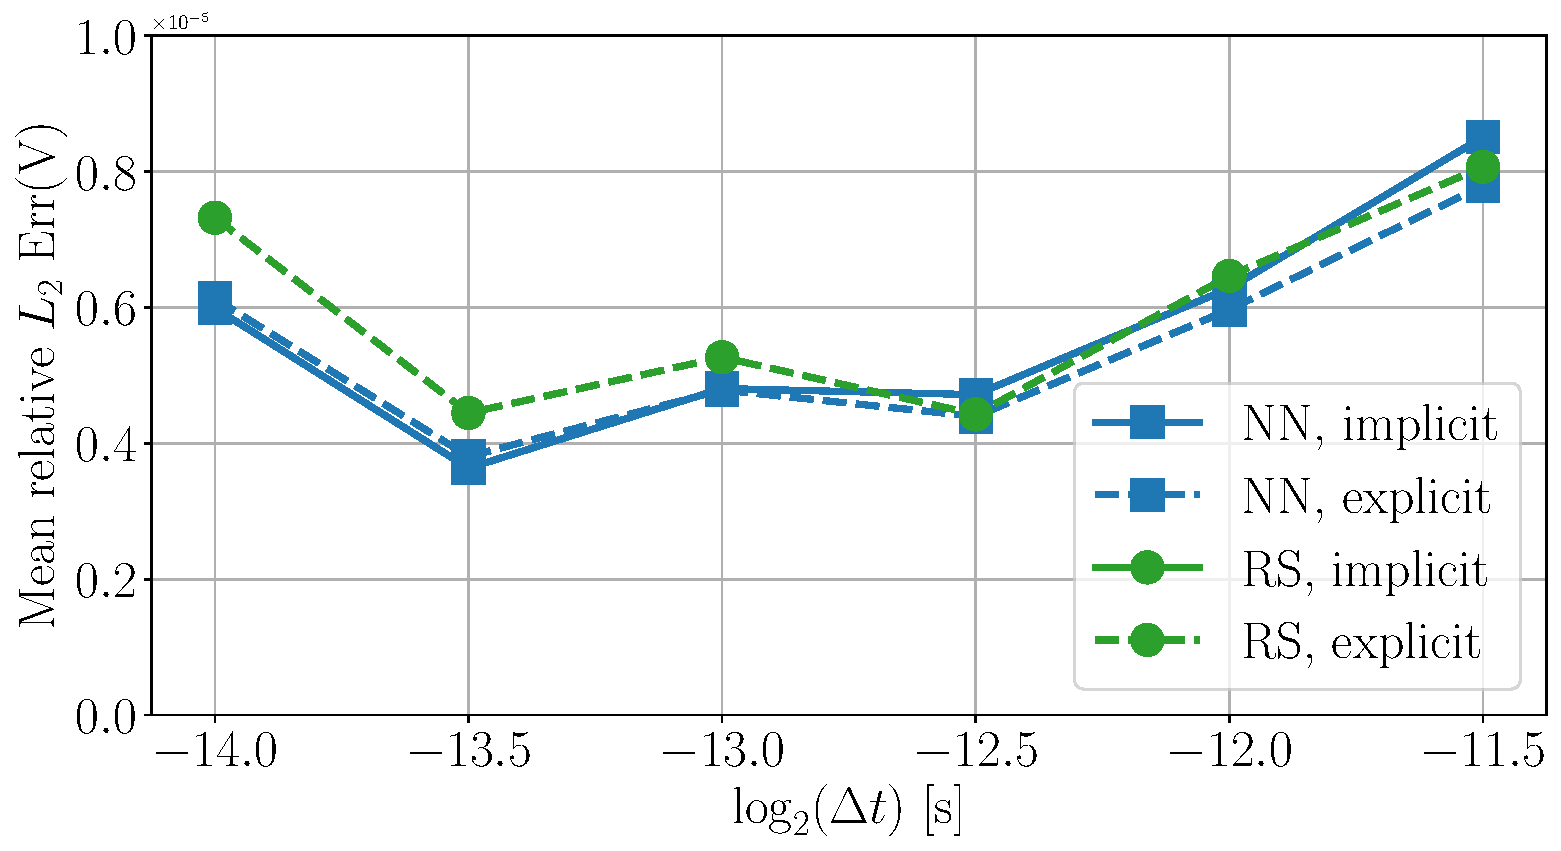
\includegraphics[width=0.7\textwidth]{figures/ErrGrowthDeltaT.pdf}
    \caption{Growth of relative $L_2$ error in $\dot{x}(t)$ as $\Delta t$ increases. 
    Note that since (RS, implicit) cannot solve some of the sequences that the other three pairs can solve, 
    its error is not plotted here.}
    \label{fig:ErrGrowthDt}
\end{figure}

